\documentclass[11pt,aspectratio=169]{beamer}

\usepackage{slides}
\usepackage{soul}
\usepackage{pdfpc}
\usepackage{ebproof}
\usepackage{bigdelim}
\usepackage{booktabs}
\usepackage{listings}
\usepackage{tcolorbox}
\usepackage{tabularx}
\usepackage{tikz}
\usepackage{xspace}
\usepackage[T1]{fontenc}
\usepackage[utf8]{inputenc}
\usepackage[symbol]{footmisc}
\usepackage[noend]{algpseudocode}
\usepackage[
    backend    = biber,
    style      = alphabetic,
    giveninits = true,
    maxnames   = 16,
    minnames   = 16,
]{biblatex}

\addbibresource{./references.bib}

\usetikzlibrary{
    positioning,
    shapes.symbols,
    shadows,
    arrows,
    calc
}

\newcommand{\senc}{\text{senc}}
\newcommand{\msg}{\text{msg}}
\newcommand{\nonce}{\text{nonce}}
\newcommand{\KDF}{\text{KDF}}
\newcommand{\key}{\text{key}}

\newcommand{\Tamarin}[1]{\textsc{Tamarin}\xspace}

%% Print: [#1] -[#2]-> [#3]
\newcommand{\MSR}[3]{#1 -\hspace{-4pt}[\hspace{5pt} #2 \hspace{4pt}]\hspace{-4.6pt}\rightarrow #3}
%% Print: -[#1]->
\newcommand{\ActionFact}[1]{-\hspace{-4pt}[\hspace{5pt} #1 \hspace{4pt}]\hspace{-4.6pt}\rightarrow}
%% Print: ~
\newcommand{\tildelow}{\raisebox{0.5ex}{\texttildelow}}
%% Print: ^
\newcommand{\pow}{\textasciicircum{}}
%% Highlight text in overlay
\newcommand{\althl}[2][2]{\alt<#1>{\hl{#2}}{#2}}

%% Sticky notes to represent facts
\definecolor{StickyNoteYellow}{RGB}{241,239,161}
\definecolor{StickyNoteRed}{RGB}{255,167,169}
\definecolor{StickyNoteGreen}{RGB}{148,199,146}
\definecolor{StickyNoteBlue}{RGB}{167,229,241}
\NewDocumentCommand{\StickyNote}{O{StickyNoteYellow}O{1cm}m}{%
    \begin{tikzpicture}
        \node[
            drop shadow={
                shadow xshift = 2pt,
                shadow yshift = -4pt,
            },
            xslant = -0.1,
            yslant = 0.1,
            draw   = black,
            fill   = #1,
            text   = black,
        ] {\parbox[t][#2][c]{#2}{\centering#3}};
    \end{tikzpicture}
}

%% Colors for terms and facts
\definecolor{TermBlue}{HTML}{1C377D}
\definecolor{FactPurple}{HTML}{7C3655}

\newcommand{\term}[1]{\textcolor{TermBlue}{#1}}
\newcommand{\Term}[1]{\textcolor{TermBlue}{#1}}
\newcommand{\Fact}[1]{\textcolor{FactPurple}{#1}}

%% Other colors
\definecolor{AdversaryRed}{HTML}{DA3B26}

%% Listings
\lstset{escapeinside={(*@}{@*)}}
\lstset{numberstyle=\tiny}

\definecolor{TamarinBlue}{RGB}{42,0,255}
\definecolor{TamarinGreen}{RGB}{48,110,32}
\definecolor{TamarinPurple}{RGB}{175,36,67}

\lstdefinestyle{tamarin}{
    basicstyle    = \linespread{0.75}\footnotesize\ttfamily,
    extendedchars = true,
    tabsize       = 2,
    columns       = fixed,
    numbers       = none,
    breaklines    = true,
    literate      = {~}{{\raisebox{0.5ex}{\texttildelow}}}{1},
    morekeywords  = {theory, builtins, restriction, equations, functions, rule,
                     let, in, lemma, All, Ex, not, predicates, begin, end},
    keywordstyle  = \color{TamarinPurple},
    morecomment   = [l]{//},
    morecomment   = [s]{/*}{*/},
    commentstyle  = \color{TamarinGreen},
    xleftmargin   = 0mm,
    upquote       = true,
    morestring    = *[b]",
    showstringspaces = false
}

\lstdefinestyle{tactic}{
    basicstyle    = \linespread{0.75}\footnotesize\ttfamily,
    extendedchars = true,
    tabsize       = 2,
    columns       = fixed,
    numbers       = none,
    breaklines    = true,
    literate      = {~}{{\raisebox{0.5ex}{\texttildelow}}}{1},
    alsoletter    = :,
    morekeywords  = {tactic:, presort:, prio:, deprio:},
    keywordstyle  = \color{TamarinPurple},
    morecomment   = [l]{//},
    morecomment   = [s]{/*}{*/},
    commentstyle  = \color{TamarinGreen},
    xleftmargin   = 0mm,
    upquote       = true,
    morestring    = *[b]",
}

\lstdefinestyle{oracle}{
    basicstyle    = \linespread{0.75}\footnotesize\ttfamily,
    extendedchars = true,
    tabsize       = 2,
    columns       = fixed,
    numbers       = none,
    breaklines    = true,
    literate      = {~}{{\raisebox{0.5ex}{\texttildelow}}}{1},
    morecomment   = [l]{\#},
    morekeywords  = {import, for, in, if, elif},
    keywordstyle  = \color{TamarinPurple},
    commentstyle  = \color{TamarinGreen},
    xleftmargin   = 0mm,
    upquote       = true,
}

\definecolor{ProVerifGreen}{RGB}{48,110,32}
\definecolor{ProVerifBlue}{RGB}{64,112,161}

\lstdefinestyle{proverif}{
    basicstyle    = \linespread{0.75}\footnotesize\ttfamily,
    extendedchars = true,
    tabsize       = 2,
    columns       = fixed,
    numbers       = none,
    breaklines    = true,
    literate      = {~}{{\raisebox{0.5ex}{\texttildelow}}}{1},
    morecomment   = [s]{(*}{*)},
    commentstyle  = \color{ProVerifGreen},
    keywordstyle  = \color{ProVerifBlue},
    morekeywords  = {in, if, event, new, let, out},
    xleftmargin   = 0mm,
}

\definecolor{proofTreeBlue}{HTML}{2639B0}
\definecolor{proofTreeRed}{HTML}{921C12}

\lstdefinestyle{prooftree}{
    basicstyle    = \linespread{0.8}\footnotesize\fontfamily{pcr}\selectfont,
    extendedchars = true,
    tabsize       = 2,
    columns       = fixed,
    numbers       = left,
    breaklines    = true,
    literate      = {~}{{\raisebox{0.5ex}{\texttildelow}}}{1},
    keywords      = [1]{lemma, case, next, qed, by, end, Diff-Lemmas},
    keywordstyle  = [1]\color{black}\bfseries,
    keywords      = [2]{simplify, solve, sorry, contradiction, induction,
                        autoprove, rule-equivalence},
    keywordstyle  = [2]\color{proofTreeBlue}\bfseries,
    keywords      = [3]{@, \|, <, \^},
    keywordstyle  = [3]\color{proofTreeRed},
    alsoletter    = @\|<\^-,
    moredelim     = **[is][{\color{proofTreeBlue}}]{<<}{>>},
    xleftmargin   = 0mm,
    upquote       = true,
    morestring    = *[b]",
}

%% Color boxes
\definecolor{ColorBoxBlue}{HTML}{1C377D}
\tcbset{
    colback      = white,
    colframe     = black,
    fonttitle    = \bfseries,
    coltitle     = white,
    colbacktitle = ColorBoxBlue,
    boxrule      = 1pt
}

%% Vertical separator for frames
\newcommand<>{\vsep}{
    \begin{tikzpicture}[remember picture,overlay]%
        \draw[ultra thick]
            ($(current page.north west)+(8cm,0.5cm)$) to
            ($(current page.south west)+(8cm,-0.5cm)$)
        ;
    \end{tikzpicture}%
}

%% Horizontal separator for frames
\newcommand<>{\hsep}{
    \begin{tikzpicture}[remember picture,overlay]%
        \draw[ultra thick]
            ($(current page.north west)+(-0.5cm,-4.5cm)$) to
            ($(current page.north east)+(0.5cm,-4.5cm)$)
        ;
    \end{tikzpicture}%
}


\title{Formal Analysis of Real-World Security Protocols}
\subtitle{Lecture 9: Advanced Features (Part 2)}
\date{\today}
\author{Aleksi Peltonen}
\institute{CISPA Helmholtz Center for Information Security}

\begin{document}
\maketitle

% ---------------------------------------------------------------------------- %
% Content
% ---------------------------------------------------------------------------- %

\begin{frame}[fragile]{Recap: Tamarin workflow}
    \begin{figure}
        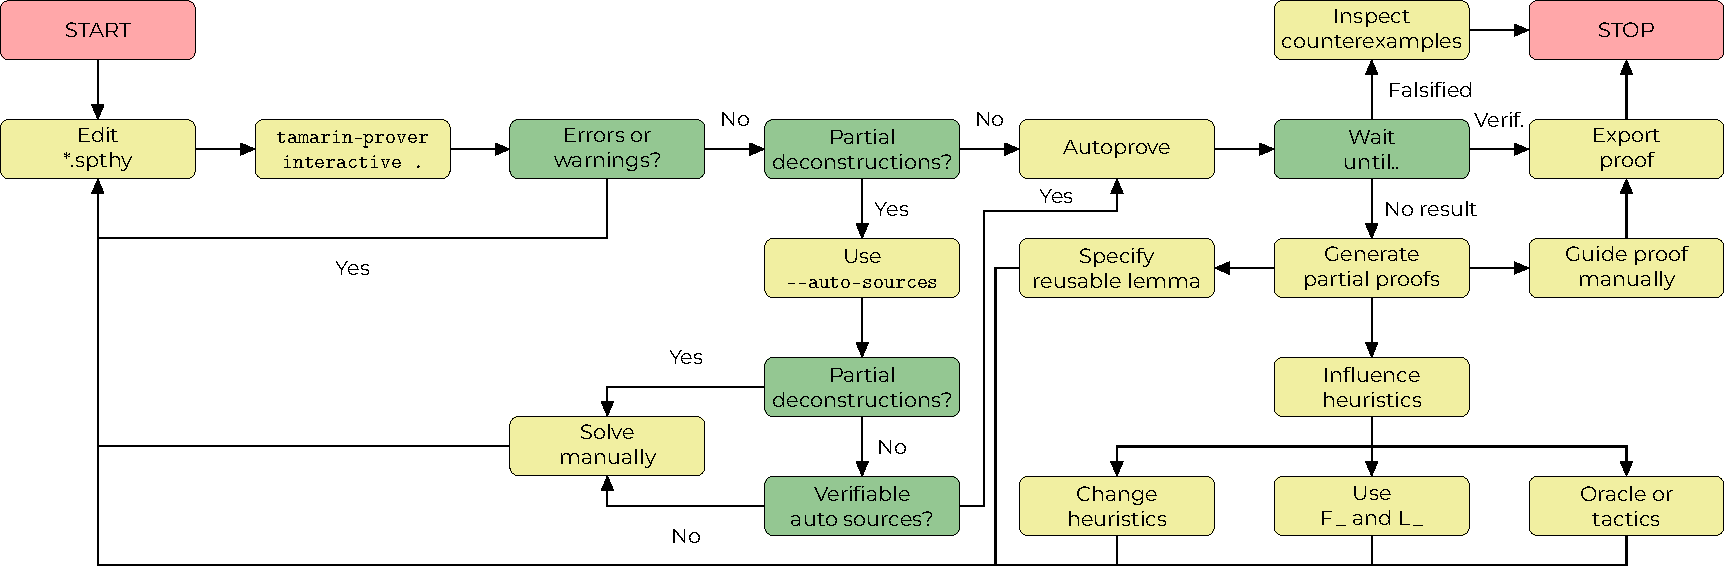
\includegraphics[width=\textwidth]{./figures/lecture_9/workflow_gui}
    \end{figure}
\end{frame}

\begin{frame}[fragile]{This lecture}
    \tableofcontents
\end{frame}

% ---------------------------------------------------------------------------- %

\section{Reducing Proof-Construction Time}

% ---------------------------------------------------------------------------- %

\begin{frame}[fragile]{Heuristics}
    \begin{tikzpicture}[remember picture,overlay]
        \node[xshift=0cm,yshift=0cm] at (current page.center){
            \includegraphics<1>[width=.9\textwidth]
                {figures/lecture_9/tamarin_gui_1.png}%
            \includegraphics<2>[width=.9\textwidth]
                {figures/lecture_9/tamarin_gui_2.png}%
        };
    \end{tikzpicture}
\end{frame}

\begin{frame}[fragile]{Heuristics}
    \begin{itemize}
        \item At any given proof step, there may be multiple open goals
        \item Tamarin uses \textbf{heuristics} to decide which goal to solve 
              first
        \item Heuristics play an important role in whether Tamarin terminates 
              and, if it does, \textbf{how quickly}
        \item However, they have \textbf{no influence on correctness}; the 
              constraint reduction steps are sound and complete
        \item Any conclusion that Tamarin reaches is always correct, regardless 
              of the proof steps taken
    \end{itemize}
\end{frame}

\begin{frame}[fragile]{Heuristics}
    \begin{itemize}
        \item Heuristics can be specified in three ways (with
              \textbf{decreasing} priority):
        \begin{enumerate}
            \item CLI argument: \verb|--heuristic=h|
            \item Lemma annotations: \verb|lemma example [heuristic=h]|
            \item Global choice for the input file: \verb|heuristic:h|
        \end{enumerate}
        \item If none of the above are chosen, Tamarin uses the
              \textbf{default heuristic}
        \item It is possible to provide several heuristic flags
        \begin{itemize}
            \item Tamarin employs a round-robin fashion depending on the proof 
                  depth
            \item e.g., \verb|--heuristic=xyy| tells Tamarin to first use 
                  heuristic \verb|x|, followed by heuristic \verb|y| twice
        \end{itemize}
        \item Tamarin defines several \textbf{built-in heuristics}
    \end{itemize}
\end{frame}

\begin{frame}[fragile]{Heuristics}
    \begin{enumerate}
        \item \textbf{smart} (\verb|--heuristic=s|)
        \begin{itemize}
            \item Works often well; \textbf{worth trying first}
            \item Prioritizes chain constraints, disjunctions, premise 
                  constraints, action constraints, and adversary knowledge that 
                  includes private or fresh terms (in this order),
                  \textit{loop breakers are delayed}
            \item If called with \verb|--heuristic=S|,
                  \textit{loop breakers are not delayed}
        \end{itemize}
        \item \textbf{consecutive/conservative} (\verb|--heuristic=c|)
        \begin{itemize}
            \item Solves goals in the order they are generated,
                  \textbf{ensuring that no goal is delayed indefinitely}
            \item Often inefficient because unimportant goals can be solved 
                  early
            \item Can sometimes \textbf{break loops} that the smart heuristic 
                  cannot
            \item Loop breakers are delayed, unless called with
                  \verb|--heuristic=C|
        \end{itemize}
    \end{enumerate}
\end{frame}

\begin{frame}[fragile]{Heuristics}
    \begin{enumerate}
        \item[3.] \textbf{injective} (\verb|--heuristic=i|)
        \begin{itemize}
            \item Specifically for protocols with \textbf{injective facts}
            \item Applies the same priorities as the smart heuristic, but 
                  instead of a strict priority hierarchy, the fact, action, and 
                  knowledge goals are considered to have equal priority and 
                  solved in the order of their creation time
            \item Rationale: For stateful protocols with an unbounded number of 
                  runs, solving a fact goal may create a new fact goal for the 
                  previous protocol run. It then makes sense to prioritize 
                  existing fact, action, and knowledge goals before solving the 
                  fact goal of that previous run, as solving that goal will 
                  likely create yet another earlier fact goal and so on, 
                  resulting in a loop
            \item Again, there is a variant that does not delay loop breakers
        \end{itemize}
    \end{enumerate}
\end{frame}

\begin{frame}[fragile]{Fact priorities}
    \begin{itemize}
        \item You can change the priority of a specific \textbf{fact} by adding 
              the prefix \verb|F_| or \verb|L_| to to its name
        \begin{itemize}
            \item Facts starting with \verb|F_| are solved \textit{first}
                  (i.e., \textbf{prioritized})
            \item Facts starting with \verb|L_| are solved \textit{last}
                  (i.e., \textbf{deprioritized})
        \end{itemize}
        \item Note: The prefix is considered to be part of the fact's name
        \begin{itemize}
            \item \verb|F_Example()| and \verb|Example()| are two different 
                  facts
        \end{itemize}
        \item You can use this to
              \textbf{ensure unrolling prefixes of relevant rules}
        \begin{itemize}
            \item The state facts needed for a rule to fire can be prioritized 
            over all others
        \end{itemize}
        \item Similarly, it can be used to \textbf{avoid} unrolling the 
              prefixes of other rules until the relevant ones are completed
    \end{itemize}
\end{frame}

\begin{frame}[fragile]{Fine-grained priorities}
    \begin{itemize}
        \item The previous option changes the priorities of facts across the 
              entire  model, i.e., \textbf{all rules} where the fact occurs
        \item In large models, we might only be interested in changing the 
              priority of specific fact instances
        \item The modifiers \verb|+| and \verb|-| can be used to modify the 
              priority of a fact \textbf{within a specific rule}
        \item Annotated in square brackets after the fact name:
        \begin{itemize}
            \item[] \verb|Fact(x)| has normal priority
            \item[] \verb|Fact(x)[+]| has high priority
            \item[] \verb|Fact(x)(-)| has low priority
        \end{itemize}
        \item Note: Unlike \verb|F_| and \verb|L_|, \verb|[+]| and \verb|[-]| 
              are not part of the fact's name
        \item Can be used for both \textbf{state facts} and
              \textbf{action facts}
    \end{itemize}
\end{frame}

\begin{frame}[fragile,t]{Custom heuristics}
    \begin{itemize}
        \item For complex proofs, we can often beat Tamarin's built-in 
              heuristic by writing our own, \textbf{model-specific heuristics}
        \item To demonstrate their use, we will use the following (artificial) 
              protocol as an example. It does not terminate at all with the 
              smart heuristic and terminates in 162 steps with the consecutive 
              (c) heuristic
    \end{itemize}
    \vspace*{.25cm}
    \lstinputlisting [
        style = tamarin,
        numbers = left,
        xleftmargin = 1.1cm,
        firstline = 8,
        lastline = 18,
    ] {./models/heuristics_example.spthy}
\end{frame}

\begin{frame}[fragile]{Custom heuristics}
    \vspace*{.5cm}
    \lstinputlisting [
        style = tamarin,
        numbers = left,
        firstline = 20,
        lastline = 40,
        firstnumber = 12,
        xleftmargin = 1.1cm,
    ] {./models/heuristics_example.spthy}
\end{frame}

\begin{frame}[fragile]{Option 1: Oracles}
    \begin{itemize}
        \item Oracles are \textbf{external Python scripts} that modify the
              order in which Tamarin applies proof steps
        \item CLI: \verb|--heuristic=O --oraclename=FILE| (default: ./oracle)
        \item During each proof step, Tamarin provides the oracle a list of 
              possible next proof steps for the current subgoal
        \item The oracle returns a sequence of numbers that \textbf{reorder} 
              some subset of the proof steps
        \begin{itemize}
            \item The reordered goals are given the \textbf{highest} priority
            \item All remaining proof steps are appended at the end in the 
                  default order
        \end{itemize}
    \end{itemize}
\end{frame}

\begin{frame}[fragile]{Option 1: Oracles}
    \begin{itemize}
        \item For example, assume that Tamarin currently has five possible 
              proof steps, initially ordered [1, 2, 3, 4, 5]
        \begin{itemize}
            \item The oracle decides that step three is the best and step two 
                  is the second best option, and returns the sequence [3, 2] to 
                  Tamarin
            \item Tamarin re-orders the proof steps to [3, 2, 1, 4, 5]
        \end{itemize}
        \item Oracles \textbf{cannot suppress proof steps and therefore do not 
              affect the correctness of the end result!}
        \begin{itemize}
            \item They can, however, cause (or fix) non-termination
        \end{itemize}
        \item Since oracles are external scripts, you can change them while 
              proving lemmas
    \end{itemize}
\end{frame}

\begin{frame}[fragile,t]{Oracle example}
    \vsep
    \vspace*{-.5cm}
    \begin{columns}[T]
        \begin{column}{0.5\textwidth}
            \lstinputlisting [
                style = oracle,
                numbers = left,
                firstline = 1,
                lastline = 20,
            ] {./models/oracle}
        \end{column}
        \begin{column}{0.5\textwidth}
            \lstinputlisting [
                style = oracle,
                numbers = left,
                xleftmargin = .5cm,
                firstline = 21,
                firstnumber = 21,
                lastline = 42,
            ] {./models/oracle}
        \end{column}
    \end{columns}
\end{frame}

\begin{frame}[fragile]{Option 2: Tactics}
    \begin{itemize}
        \item Tactics are a \textbf{built-in language} for specifying custom 
              heuristics
        \item Tactics can be called like built-in heuristics:
        \begin{itemize}
            \item CLI argument: \verb|--heuristic={tacticName}|
            \item Lemma annotations:
                  \verb|lemma example [heuristic={tacticName}]|
            \item Global choice for the input file:
                  \verb|heuristic:{tacticName}|
        \end{itemize}
        \item You can write tactics directly in the \verb|.spthy| file, or 
              include a separate file with the pre-processor command
              \verb|#include|
        \item Goals that are not ranked with a tactic are kept in their 
              original order and inserted \textbf{between} the facts that are 
              ranked
    \end{itemize}
\end{frame}

\begin{frame}[fragile,t]{Option 2: Tactics}
    \vsep
    \vspace*{-.8cm}
    \begin{columns}[T]
        \begin{column}{0.5\textwidth}
            \begin{itemize}
                \item \textbf{Syntax:}
            \end{itemize}
            \vspace*{.15cm}
            \begin{lstlisting}[
                style = tactic,
                gobble = 16,
                xleftmargin = 1cm,
            ]
                tactic: example
                presort: heuristic
                prio:
                    selectionFun1 "arg1"
                prio:
                    selectionFun2 "arg2"
                deprio:
                    selectionFun3 "arg3"
            \end{lstlisting}

            \begin{itemize}
                \item Goals matching the first \verb|prio| have the
                      \textbf{highest priority}
                \item Goals matching the last \verb|deprio| have the
                      \textbf{lowest priority}
            \end{itemize}
        \end{column}
        \begin{column}{0.5\textwidth}

            The goals are ordered as follows:
            \begin{enumerate}
                \item All goals matching selectionFun1 ``arg1''
                \item All goals matching selectionFun2 ``arg2''
                \item All goals matching \textbf{none} of the
                      \verb|prio| or \verb|deprio| selections
                \item All goals matching selectionFun3 ``arg3''
            \end{enumerate}
        \end{column}
    \end{columns}
\end{frame}

\begin{frame}[fragile]{Option 2: Tactics}
    \begin{itemize}
        \item Selection functions:
        \begin{enumerate}
            \item \textbf{regex}
                  (e.g., \verb|regex "Fact_1\( |\tildelow{}\verb|id"|))
            \begin{itemize}
                \item Takes as an argument a string, which is interpreted as a 
                      regular expression and matched against the string 
                      representation of the goal
                \item If the match succeeds, the goal is selected
            \end{itemize}
            \item \textbf{isFactName} (e.g., \verb|isFactName "Fact_1"|)
            \begin{itemize}
                \item Takes as an argument a string, which is interpreted as a 
                      fact name
                \item Selects premise goals that require a fact of this name
            \end{itemize}
            \item \textbf{isInFactTerms}
                  (e.g., \verb|isInFactTerms "|\tildelow{}\verb|id"|)
            \begin{itemize}
                \item Takes as an argument a string, which is interpreted as a 
                      regular expression
                \item Selects action goals that contain a term matching the 
                      regular expression
            \end{itemize}
        \end{enumerate}
    \end{itemize}
\end{frame}

\begin{frame}[fragile]{Oracles or tactics?}
    \begin{itemize}
        \item We can rewrite the \textbf{40-line oracle} as an
              \textbf{8-line tactic}:
        \vspace*{.25cm}
        \lstinputlisting [
            style = tactic,
            numbers = left,
            xleftmargin = .5cm,
        ] {./models/tactic}
        \item Both reduce the proof from \textbf{162 steps to 10}
        \item Tactics are pre-processed with the model, oracles can be edited 
              while proving
        \begin{itemize}
            \item ..but they have an external dependency (Python), which
                  \textbf{might cause problems with reproducibility}
        \end{itemize}
    \end{itemize}
\end{frame}

% ---------------------------------------------------------------------------- %
% Reading Material
% ---------------------------------------------------------------------------- %
\begin{frame}[fragile]{Reading material}
    \textbf{Recommended reading}:
        ~\cite[Ch. 16]{tamarin-book}
    \printbibliography[heading=none]
\end{frame}
% ---------------------------------------------------------------------------- %

\end{document}
